\section{Transient Performance of Multi Machine Lines}
\noindent In this section we extend the two-machine model to multi-machine model. The model now can be used with arbitrary numbers of machines and buffers composition. The importanet problem that we need to solve, is to arrange the operations that in one time slot the machines and buffers should do.

\subsection{Mathematical Dirivation of multi-machine Model}
\noindent Suppose we have an $M$-machine geometric line observing assumptions 1-8. Because the geometric distribution obey the memoryless attribute, the system can still be described by a Markov chain. Use $j_i(n)$ to indicate the number of parts in buffer $b_i$ at the start of time slot $n$. Moreover, we can describe the state of Markov chain with vector $(j_1(n), ... , j_{M-1}(n)$, $ s_1(n), ..., s_M(n))$, where $j_i(n) \in {0, 1, ...,N_i}, i = 1, ..., M-1$, and $s_i(n) \in {0, 1}, i = 1, ..., M$. Apparently, the system has totally states of $S = 2^M \sum^{M-1}_{i=1} (N_i + 1)$. To derive the transition probabilities among these states, the same approach described in Section \ref{mathematical two machine} is applied to linearize the state space. Particularly, the states from State 1 to S are arranged in the following manner: $r(j_1, ..., j_{M-1}, s_1, ..., s_M)$ refer to the state number of the Markov chain state $(j_1, ..., j_{M-1}, s_1, ..., s_M)$. Define
\begin{equation}
    r(j_1,...,j_{M-1},s_1,...,s_m) = 1+\sum^{M-1}_{i=1}j_i\alpha _i + \sum^M_{i=1}s_i\beta _i
    \label{multimachine r}
\end{equation}
where
\begin{align*}
    \alpha_i &= \left\{ 
      \begin{aligned} &2^M \ \prod^{M-1}_{h=i+1}(N_h + 1),  &i &= 1,...,M-2 \\ &2^M \ , &i &= M-1 
      \end{aligned}
    \right. 
    \\ \beta _i &= 2^{M-1}, i = 1,...,M
  \end{align*}
  In this regulation, each state can be arranged a individual number between 1 and S. On the contrary, consider the state number $r$ of a system state, $r\in{1, .., S}$, the corresponding machine state $s^{(r)}_i ,  i = 1, ..., M$, and buffer state, $j^{(r)}_i , i = 1,..., M-1$, can be derived as follows:

\begin{equation}
    j^{(r)}_i = \left\{
\begin{aligned}
    &\lf{\frac{r-1}{\alpha_1}}\rf, &i&=1 \\ &\lf{\frac{r-1-\sum^{i-1}_{h-1}j^{(r)}_h\alpha_h}{\alpha_i}}\rf, &i&=2,...,M-1
\end{aligned}    
\right.
\end{equation}

\begin{equation}
    s_i^{(r)}=\left\{
    \begin{aligned}
        &\lf{\frac{r-1-\sum^{M-1}_{h-1}j^{(r)}_h\alpha_h}{\beta_1}}\rf, &i&=1 \\ &\lf{\frac{r-1-\sum^{M-1}_{h-1}j^{(r)}_h\alpha_h-\sum^{i-1}_{h-1}s^{(r)}_h\beta_h}{\beta_i}}\rf, &i&=2,...,M
    \end{aligned}\right.
\end{equation}

As is shown above, compared to the two-machine production lines model, the state arrangement of both system are very similar, but in this term with enlarged state it can accomodate more buffers and machines.

Alike with the two-machine situation, the transitions of $j_i(n)$'s are deterministic with machine state $s_1(n),...,s_M(n)$, and can be computed according to the following equations:
\begin{equation}
    \begin{aligned}
      j_i(n + 1) &= j'_i(n) + s_i(n)min\{j_{i-1}(n),N_i - j'_i(n), 1\} \\
      i &= 2, ..., M - 1 \\
      j_1(n + 1) &= j'_1(n) + s_1(n)min\{N_1 - j'_1(n), 1\}
    \end{aligned}
    \end{equation}
    where
    \begin{equation}
      \begin{aligned}
      j'_{M-1}(n)&=j_{M-1}(n) - s_M(n)min\{j_{M-1}(n), 1\} \\
    j'_i(n)&=j_i(n)- s_{i+1}(n)min\{j_i(n),N{i+1}-j'{i+1}(n), 1\} \\
     i &= 1, . . . , M - 2.
    \end{aligned}
    \end{equation}
In the above equtions, $j'_i(n)$ indicates the occupancy of buffer $b_i$ as loog as machine $m_{i+1}$ takes a products  from $b_i$ at the start of time slot $n$.

Subsequently, according to the state number derived in \ref{multimachine r} all $S$ system states from $1$ to $S$ and describe $x_i(n) = $ Prob[System in state $i$ in time slot $n$]. Afterwards, the procedure of the state transformation of the Markov chain, $x(n) = [x_1(n)x_2(n)...x_S(n)]^T$, can be derived by
\begin{equation}
    x(n+1) = A_Mx(n), \sum^S_{i=1}x_i(n) = 1.
\end{equation}

The transient perfomrmace of the system can be given by

\begin{equation}
    \begin{aligned}
  PR(n) &= \text{Prob}[m_M \text{up and} b_{M-1} \text{not empty at time slot} n] \\
        &= \text{Prob}[s_M(n) = 1 \text{and} j_{M-1}(n) > 0] \\
        &=D_1x(n) = [d_{1,1}d_{1,2}...d_{1,S}]x(n) \\
  CR(n) &= \text{Prob}[m_1 \text{is up and not blocked at time slot} n] \\
        &= D_2x(n) = [d_{2,1}d_{2,2}...d_{2.S}]x(n) \\
WIP_i(n) &=\sum^{N_i}_{k=1}k\cdot \text{Prob}[j_i(n)=k] \\
        &= D_{3,i}x(n) = [d_{3,1}d_{3,2}...d_{3.S}]x(n), i=1,...,M-1 \\
ST_i(n) &=  \text{Prob}[m_i \text{up and} b_{i-1} \text{empty at time slot} n] \\
        &= \text{Prob}[s_i(n) = 1 \text{and} j_{i-1}(n) = 0] \\
        &= D_{4,i}x(n) = [d_{4,1}d_{4,2}...d_{4.S}]x(n), i=2,...,M \\
BL_i(n) &=  \text{Prob}[m_i \text{up} b_{i} \text{full, and} m_{i+1}\text{down or blocked at time slot} n] \\
        &= D_{5,i}x(n) = [d_{5,1}d_{5,2}...d_{5.S}]x(n), i=1,...,M-1
     \end{aligned}
\end{equation}
where
\begin{align*}
    d_{1,r} &= \left\{\begin{aligned}  &1, \text{if}s^{(r)}_M = 1 \text{and} j^{(r)}_{M-1}  > 0 \\ &0, otherwise
    \end{aligned}\right. \\
    d_{2,r} &= 1- d_{5,1,r} \\
    d_{3,i,r} &= j^{(r)}_i, i = 1,...,M-1,  r = 1,...,S \\
    d_{4,i,r} &= \left\{\begin{aligned} &1, \text{if} s^{(r)}_i = 1 \text{and} j^{(r)}_{i-1}=0 \\ &0 , otherwise
    \end{aligned}\right. \\
    d_{5,i,r} &= \left\{\begin{aligned} & d_{5,i+1,r},  &\text(if) s^{(r)}_i &=1,s^{(r)}_{i+1} =1, \text{and} j^{(r)}_i = N_i \\  & 1,  &\text(if) s^{(r)}_i &=1,s^{(r)}_{i+1} =0, \text{and} j^{(r)}_i = N_i \\ & 0, &otherwise
    \end{aligned}\right.
  \end{align*}
  in other words, $d_{1,r},d_{2,r}, d_{3,i,r}, d_{4,i,r}$ and $d_{5,i,r}$ represent the $r$th element in vectors $D_1,D_2,$ $D_{3,i},D_{4,i}$ and $D_{5,i}$, separately. Apparently, in system state $x(n)$ all the performance measures are linear.

  As an instance, suppose a four-machine geometric line obeying the assumptions 1-8. with machines and buffer parameters
  \begin{displaymath}
      P_i = 0.05, R_i-0.2, i = 1,...4; N_i = 5, i=1,...3.
  \end{displaymath}

  Presume that all machines are broken down in the beginning and buffers are all empty either. The transient performance of this system are shown in Figure \ref{Transients of a four-machine geometric line}.


\begin{figure*}[!h]
	\centering
	\subfigure[]{
		\includegraphics[width=0.45\linewidth,height=0.35\linewidth]{figures/four_machine_pr_and_cr.tikz}
		\label{four machine pr and cr}}
	\subfigure[]{
		\includegraphics[width=0.45\linewidth,height=0.35\linewidth]{figures/four_machine_wip.tikz}	
		 \label{four machine wip}}
	\subfigure[]{
		\includegraphics[width=0.45\linewidth,height=0.35\linewidth]{figures/four_machine_st.tikz}	
		\label{four machine st}}
	\subfigure[]{
		\includegraphics[width=0.45\linewidth,height=0.35\linewidth]{figures/four_machine_bl.tikz}	
		\label{four machine bl}}
	\caption{Transients of a four-machine geometric line. (a) $PR(n) \ and\ CR(n)$;(b) $WIP(n)$; (c) $ST_i(n)$;(d) $BL_i(n)$.}
	\label{Transients of a four-machine geometric line}
\end{figure*}

\subsection{Implementation of multi-machine model}
\noindent In the python platform, it is also very similar to two-machine model in section \ref{Transients of a four-machine geometric line}. The \pythoninline{class Individual} and \pythoninline{class Buffer} are also keeped to represent one machine instance and one buffer instance, while they are reorganized in new \pythoninline{class MultiMachine}. In addition, in each \pythoninline{MultiMachine} instance it contains two arrays named as \pythoninline{Machine} and \pythoninline{BufferArray} respectively. The formor array contains a number of \pythoninline{MachineNumber} machines while the latter array holds one less buffer compared to the formor array. 

We use a UML diagram to illustrate the relationship between these class, see Figure \ref{multi machine uml}. In script ''sim4.py'' we initialize all the given parameters and create enough instances of \pythoninline{class MultiMachine}. Therefore, in each time slot the critical transient performance measures are collected from function \pythoninline{one_slot()}, and in the end write in the file.

\begin{figure*}[!h]
	\centering
	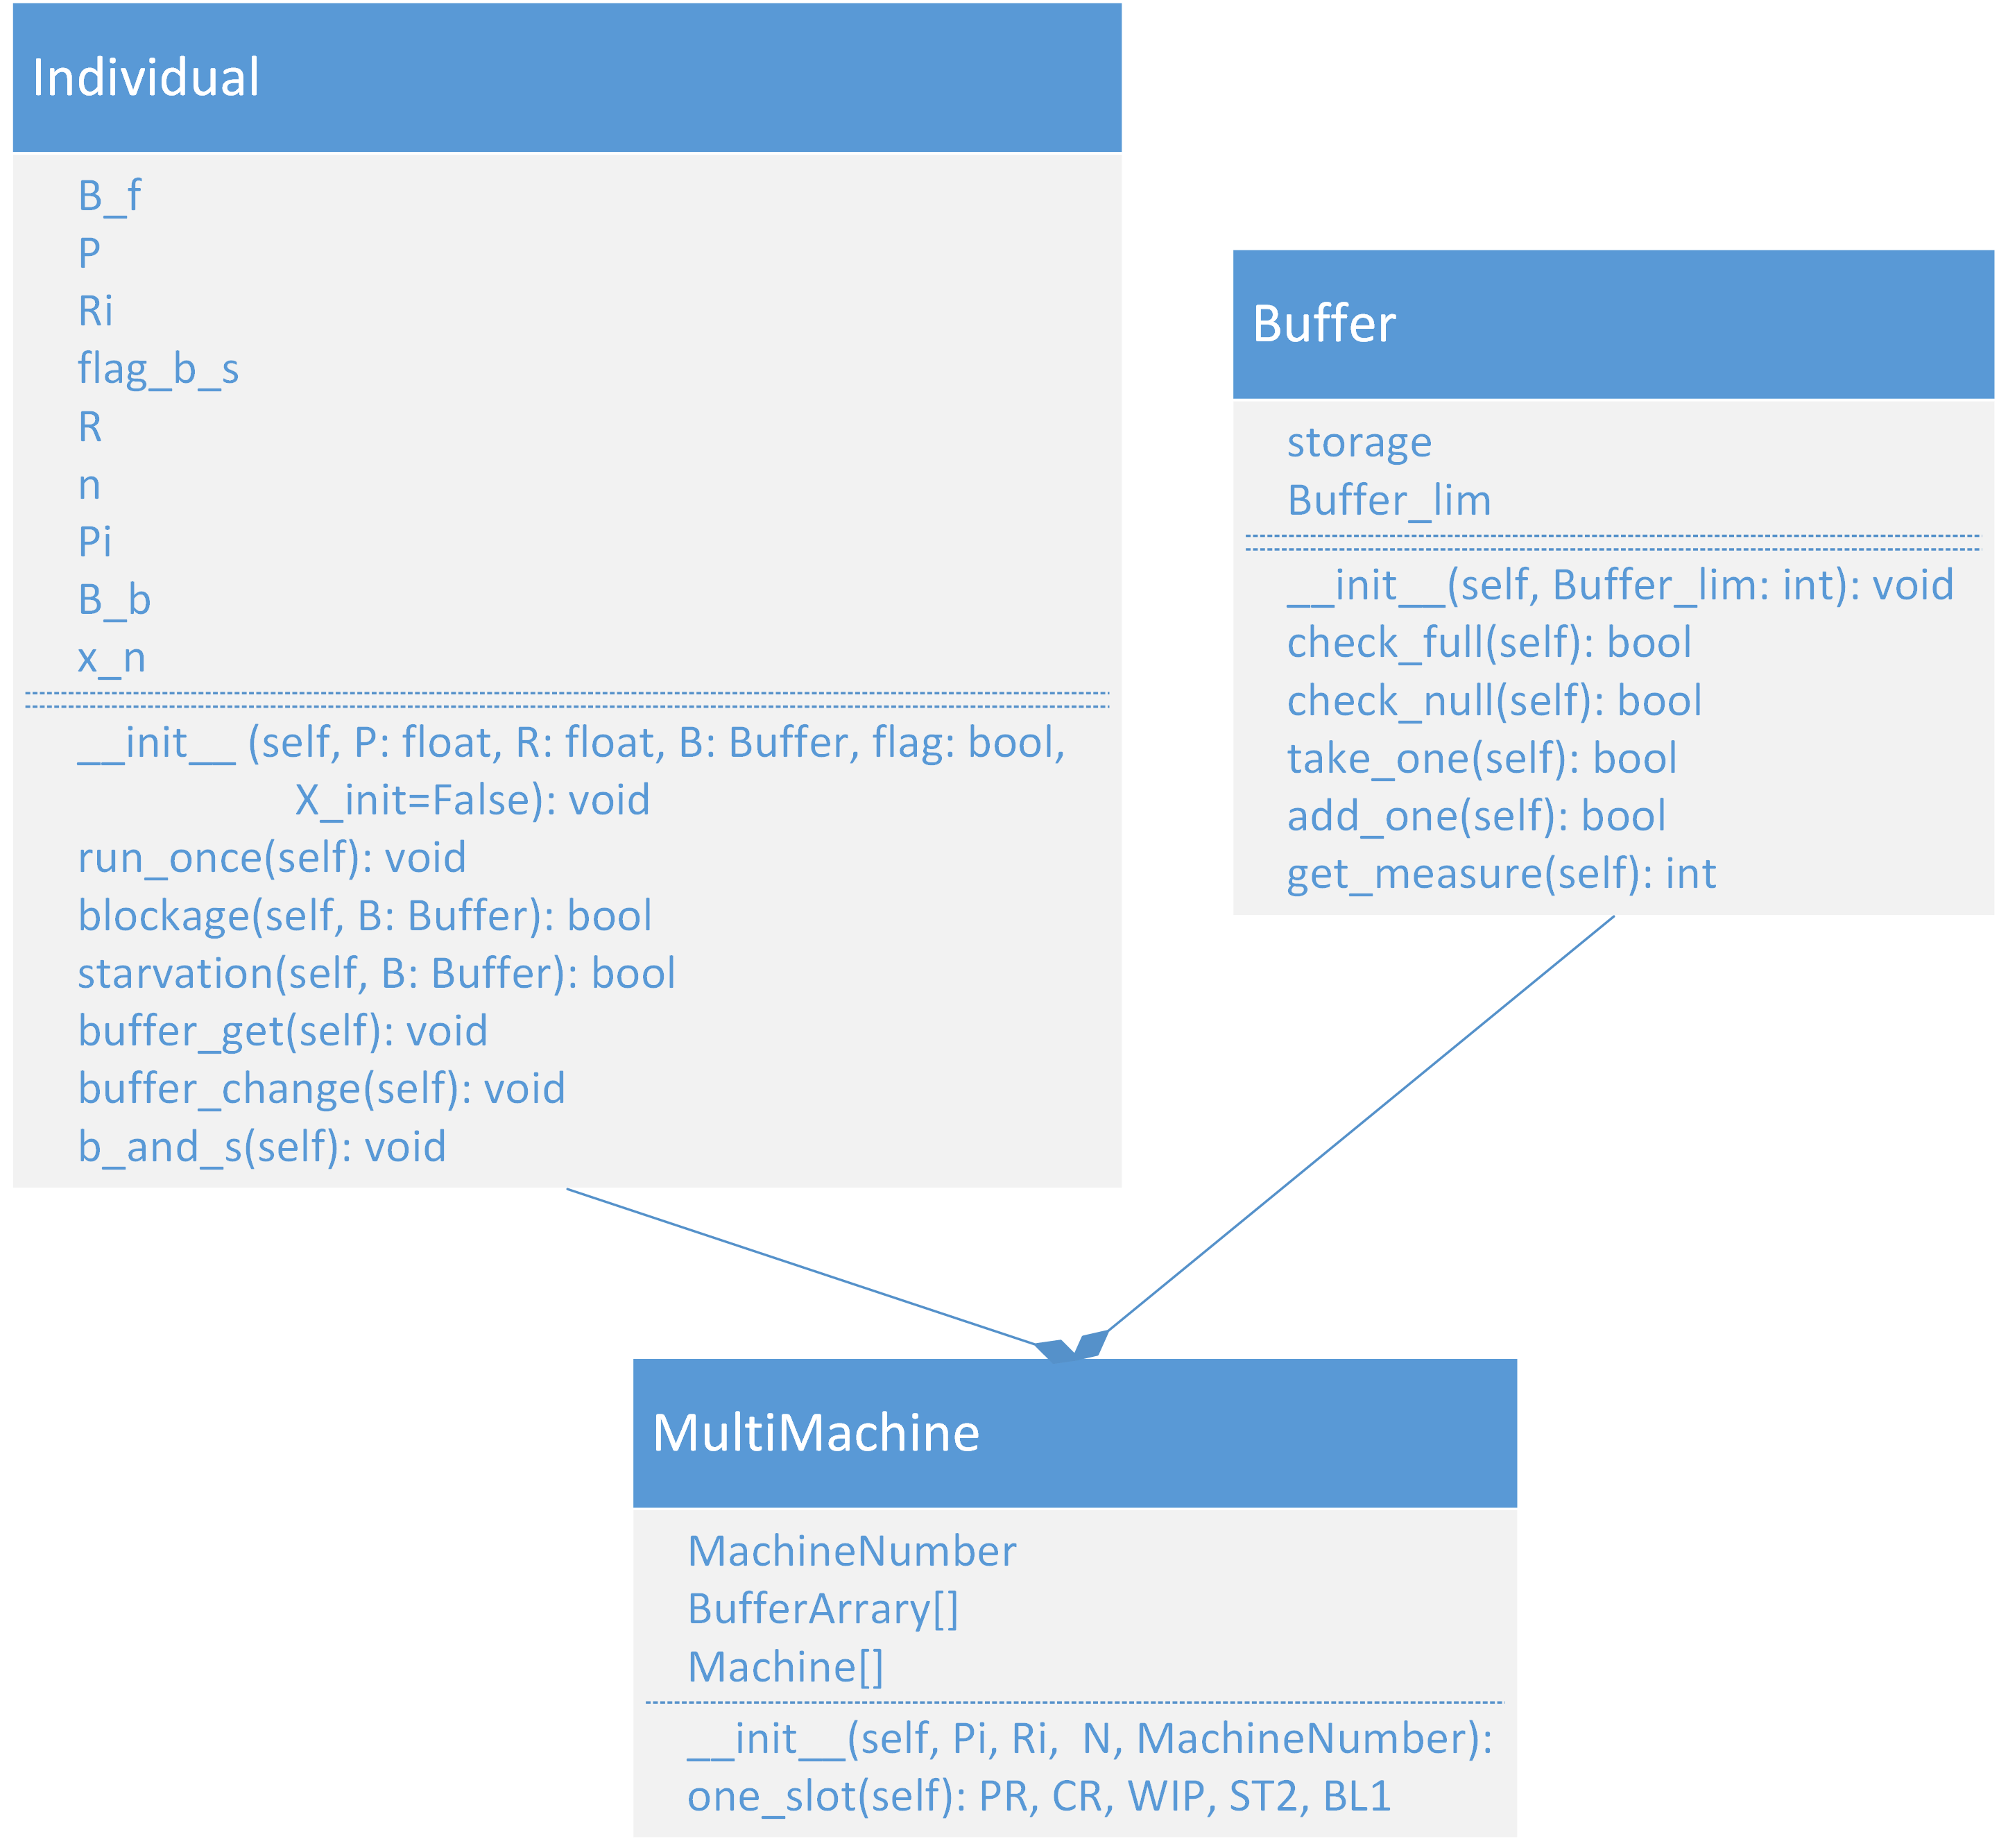
\includegraphics[width=0.8\linewidth]{multi_machine.png}
	\caption{UML diagram of a multi-machine model}
	\label{multi machine uml}
\end{figure*}